\documentclass{beamer}
\usepackage{amsmath}
\usepackage[english]{babel} %set language; note: after changing this, you need to delete all auxiliary files to recompile
\usepackage[utf8]{inputenc} %define file encoding; latin1 is the other often used option
\usepackage{csquotes} % provides context sensitive quotation facilities
\usepackage{graphicx} %allows for inserting figures
\usepackage{booktabs} % for table formatting without vertical lines
\usepackage{textcomp} % allow for example using the Euro sign with \texteuro
\usepackage{stackengine}
\usepackage{wasysym}
\usepackage{tikzsymbols}
\usepackage{textcomp}
\usepackage{xcolor}
\usepackage[dvipsnames]{xcolor}
\usepackage{colortbl}
\usepackage{adjustbox}
\usepackage{tikz} % allows drawing figures
\usetikzlibrary{decorations.pathreplacing}
\newcommand{\bubblethis}[2]{
        \tikz[remember picture,baseline]{\node[anchor=base,inner sep=0,outer sep=0]%
        (#1) {\underline{#1}};\node[overlay,cloud callout,callout relative pointer={(0.2cm,-0.7cm)},%
        aspect=2.5,fill=yellow!90] at ($(#1.north)+(-0.5cm,1.6cm)$) {#2};}%
    }%
\tikzset{face/.style={shape=circle,minimum size=4ex,shading=radial,outer sep=0pt,
        inner color=white!50!yellow,outer color= yellow!70!orange}}
%% Some commands to make the code easier
\newcommand{\emoticon}[1][]{%
  \node[face,#1] (emoticon) {};
  %% The eyes are fixed.
  \draw[fill=white] (-1ex,0ex) ..controls (-0.5ex,0.2ex)and(0.5ex,0.2ex)..
        (1ex,0.0ex) ..controls ( 1.5ex,1.5ex)and( 0.2ex,1.7ex)..
        (0ex,0.4ex) ..controls (-0.2ex,1.7ex)and(-1.5ex,1.5ex)..
        (-1ex,0ex)--cycle;}
\newcommand{\pupils}{
  %% standard pupils
  \fill[shift={(0.5ex,0.5ex)},rotate=80] 
       (0,0) ellipse (0.3ex and 0.15ex);
  \fill[shift={(-0.5ex,0.5ex)},rotate=100] 
       (0,0) ellipse (0.3ex and 0.15ex);}

\newcommand{\emoticonname}[1]{
  \node[below=1ex of emoticon,font=\footnotesize,
        minimum width=4cm]{#1};}
\usepackage{scalerel}
\usetikzlibrary{positioning}
\usepackage{xcolor,amssymb}
\newcommand\dangersignb[1][2ex]{%
  \scaleto{\stackengine{0.3pt}{\scalebox{1.1}[.9]{%
  \color{red}$\blacktriangle$}}{\tiny\bfseries !}{O}{c}{F}{F}{L}}{#1}%
}
\newcommand\dangersignw[1][2ex]{%
  \scaleto{\stackengine{0.3pt}{\scalebox{1.1}[.9]{%
  \color{red}$\blacktriangle$}}{\color{white}\tiny\bfseries !}{O}{c}{F}{F}{L}}{#1}%
}
\usepackage{fontawesome} % Social Icons
\usepackage{epstopdf} % allow embedding eps-figures
\usepackage{tikz} % allows drawing figures
\usepackage{amsmath,amssymb,amsthm} %advanced math facilities
\usepackage{lmodern} %uses font that support italic and bold at the same time
\usepackage{hyperref}
\usepackage{tikz}
\hypersetup{
    colorlinks=true,
    linkcolor=blue,
    filecolor=magenta,      
    urlcolor=blue,
}
\usepackage{tcolorbox}
%add citation management using BibLaTeX
\usepackage[citestyle=authoryear-comp, %define style for citations
    bibstyle=authoryear-comp, %define style for bibliography
    maxbibnames=10, %maximum number of authors displayed in bibliography
    minbibnames=1, %minimum number of authors displayed in bibliography
    maxcitenames=3, %maximum number of authors displayed in citations before using et al.
    minnames=1, %maximum number of authors displayed in citations before using et al.
    datezeros=false, % do not print dates with leading zeros
    date=long, %use long formats for dates
    isbn=false,% show no ISBNs in bibliography (applies only if not a mandatory field)
    url=false,% show no urls in bibliography (applies only if not a mandatory field)
    doi=false, % show no dois in bibliography (applies only if not a mandatory field)
    eprint=false, %show no eprint-field in bibliography (applies only if not a mandatory field)
    backend=biber %use biber as the backend; backend=bibtex is less powerful, but easier to install
    ]{biblatex}
\addbibresource{../mybibfile.bib} %define bib-file located one folder higher


\usefonttheme[onlymath]{serif} %set math font to serif ones

\definecolor{beamerblue}{rgb}{0.2,0.2,0.7} %define beamerblue color for later use

%%% defines highlight command to set text blue
\newcommand{\highlight}[1]{{\color{blue}{#1}}}


%%%%%%% commands defining backup slides so that frame numbering is correct

\newcommand{\backupbegin}{
   \newcounter{framenumberappendix}
   \setcounter{framenumberappendix}{\value{framenumber}}
}
\newcommand{\backupend}{
   \addtocounter{framenumberappendix}{-\value{framenumber}}
   \addtocounter{framenumber}{\value{framenumberappendix}}
}

%%%% end of defining backup slides

%Specify figure caption, see also http://tex.stackexchange.com/questions/155738/caption-package-not-working-with-beamer
\setbeamertemplate{caption}{\insertcaption} %redefines caption to remove label "Figure".
%\setbeamerfont{caption}{size=\scriptsize,shape=\itshape,series=\bfseries} %sets figure  caption bold and italic and makes it smaller

\newtcolorbox{boxA}{
    fontupper = \bf,
    boxrule = 1.5pt,
    colframe = black % frame color
}
\newtcolorbox{boxB}{
    boxrule = 1.5pt,
    colframe = blue!70!black,, % frame color
    colback = blue!7!white,
}
\usetheme{Boadilla}

% --------------------
% Overall information
% --------------------
\title[Economía I]{Economía I \vspace{4mm}
\\ Magistral 25: Política Monetaria y Fiscal}
\date{}
\author[Franco Riottini]{Riottini Franco}
\vspace{0.4cm}
\institute[]{Universidad de San Andrés} 


\begin{document}

\begin{frame}
\titlepage
\centering

\includegraphics[scale=0.2]{../Figures/logoUDESA.jpg} 
\end{frame}

\begin{frame}{El mecano en gráficos}

\begin{itemize}
    \item Vamos a usar lo que vimos hasta ahora para darle una representación gráfica al sistema 
    \item Esto va implicar graficar conjuntamente el mercado de bienes y dinero.
    \item En los gráficos que siguen usamos la siguiente terminología, 
    \begin{itemize}
        \item \textit{P}: el nivel de precios de la economía
        \item \textit{Y}: el nivel del producto
        \item \textit{i}: la tasa de interés nominal
        \item \textit{M}: la cantidad de dinero
        \item \textit{FP}: la cantidad de crédito
    \end{itemize}
\end{itemize}

\end{frame}
\begin{frame}{El mecano en el mundo clásico}
    \begin{center}
        \begin{figure}[H]
        \renewcommand{\figurename}{Figure}
            \begin{center}
                \begin{minipage}[b]{0.45\textwidth}
                    \begin{center}
                        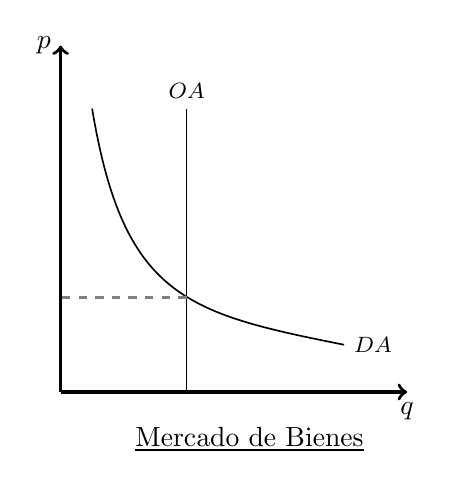
\begin{tikzpicture}[scale=0.4]
                            \draw[very thick,<-] (0,11)--(0,0);
                            \draw[very thick,->] (0,0)--(11,0) node[below]{$q$};
                            \node[left] at (0,11) {$p$};
                            \node[] at(6,-1.5) {\underline{Mercado de Bienes}};
                            \draw[semithick] (1,9).. controls (2,3) and (4, 2.5) .. (9, 1.5) node [right]{\footnotesize $DA$};
                            \draw[semithick](4, 0)--(4, 9) node [above]{\footnotesize $OA$};
                            \draw[thick, gray, dashed] (4,3)--(0,3);
                        \end{tikzpicture}
                    \end{center}
                \end{minipage}
                \begin{minipage}[b]{0.45\textwidth}
                    \begin{center}
                        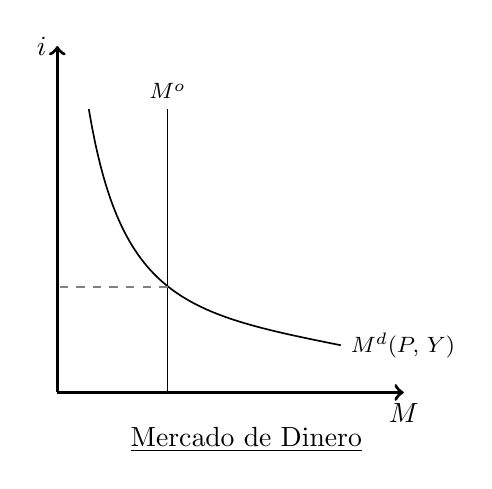
\begin{tikzpicture}[scale=0.4]
                        \draw[very thick,<-] (0,11) node[left]{$i$}--(0,0);
                        \draw[very thick,->] (0,0)--(11,0) node[below]{$M$};
                        \node[right] at (0,11) {};
                        \node[] at(6,-1.5) {\underline{Mercado de Dinero}};
                        \draw[semithick] (1,9).. controls (2,3) and (4, 2.5) .. (9, 1.5) node [right]{\footnotesize $M^{d}(P,\, Y)$};
                        \draw[semithick](3.5, 0)--(3.5, 9) node [above]{\footnotesize $M^{o}$};
                        \draw[thick, gray, dashed] (3.5,3.35)--(0,3.35);
                        \end{tikzpicture}
                    \end{center}
                \end{minipage}
            \end{center}
        \end{figure}
    \end{center} 

\end{frame}

\begin{frame}{El mecano en el mundo keynesiano}
    \begin{center}
    \begin{figure}[H]
    \renewcommand{\figurename}{Figure}
    \begin{center}
    \begin{minipage}[b]{0.45\textwidth}
    \begin{center}
    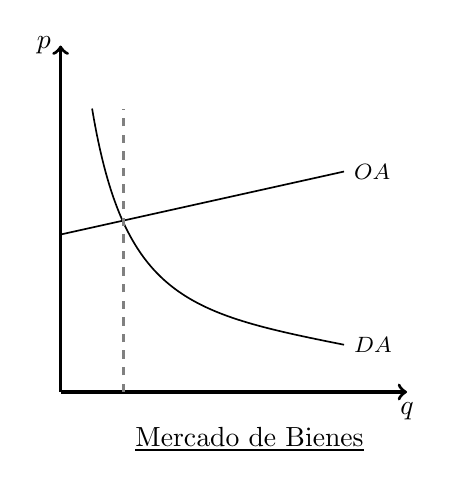
\begin{tikzpicture}[scale=0.4]
    \draw[very thick,<-] (0,11)--(0,0);
    \draw[very thick,->] (0,0)--(11,0) node[below]{$q$};
    \node[left] at (0,11) {$p$};
    \node[] at(6,-1.5) {\underline{Mercado de Bienes}};
    \draw[semithick] (1,9).. controls (2,3) and (4, 2.5) .. (9, 1.5) node [right]{\footnotesize $DA$};
    \draw[semithick](0, 5)--(9,7) node [right]{\footnotesize $OA$};
    \draw[thick, gray, dashed] (2,0)--(2,9);
    \end{tikzpicture}
    \end{center}
    \end{minipage}
    \begin{minipage}[b]{0.45\textwidth}
    \begin{center}
    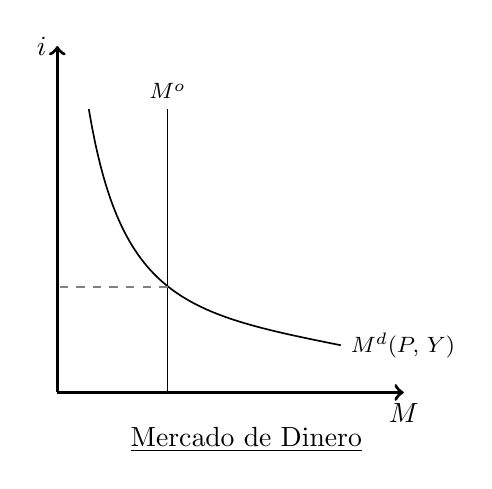
\begin{tikzpicture}[scale=0.4]
    \draw[very thick,<-] (0,11) node[left]{$i$}--(0,0);
    \draw[very thick,->] (0,0)--(11,0) node[below]{$M$};
    \node[right] at (0,11) {};
    \node[] at(6,-1.5) {\underline{Mercado de Dinero}};
    \draw[semithick] (1,9).. controls (2,3) and (4, 2.5) .. (9, 1.5) node [right]{\footnotesize $M^{d}(P,\, Y)$};
    \draw[semithick](3.5, 0)--(3.5, 9) node [above]{\footnotesize $M^{o}$};
    \draw[thick, gray, dashed] (3.5,3.35)--(0,3.35);
    \end{tikzpicture}
    \end{center}
    \end{minipage}
    \end{center}
    \end{figure}
    \end{center} 
\end{frame}

\begin{frame}{Política Monetaria en el mundo clásico}
    
    \begin{center}
    \begin{figure}[H]
    \renewcommand{\figurename}{Figure}
    \begin{center}
    \begin{minipage}[b]{0.45\textwidth}
    \begin{center}
    \begin{tikzpicture}[scale=0.4]
    \draw[very thick,<-] (0,11)--(0,0);
    \draw[very thick,->] (0,0)--(11,0) node[below]{$q$};
    \node[left] at (0,11) {$p$};
    \node[left] at (0,3) {$p_0$};
    \draw[thick, gray, dashed] (4,3)--(0,3);
    \node[] at(6,-1.5) {\underline{Mercado de Bienes}};
    \draw[semithick] (1,9).. controls (2,3) and (4, 2.5) .. (9, 1.5) node [right]{\footnotesize $DA$};
    \draw[semithick](4, 0)--(4, 9) node [above]{\footnotesize $OA$};
    \draw[thick, gray, dashed] (4,3)--(0,3);
    
    \draw[fill] (4,3) circle [radius =0.11] node[above right] {$A$};
    \only<2->{
        \draw[thick, gray, dashed] (7.5,3)--(4,3);
        \draw[fill, blue] (7.5,3) circle [radius =0.11] node[above right] {$B$};
        \draw[semithick, blue] (2.25,9).. controls (2.75,4) and (7, 3) .. (9, 2.75) node [right]{\footnotesize $DA'$};
    }
    \only<3->{
        \draw[thick, green, dashed] (4,5)--(0,5);
        \node[left, green] at (0,5) {$p_1$};
        \draw[fill, green] (4,5) circle [radius =0.11] node[above right] {$C$};
    }
    \end{tikzpicture}
    \end{center}
    \end{minipage}
    \begin{minipage}[b]{0.45\textwidth}
    \begin{center}
    \begin{tikzpicture}[scale=0.4]
    \draw[very thick,<-] (0,11) node[left]{$i$}--(0,0);
    \draw[very thick,->] (0,0)--(11,0) node[below]{$M$};
    \node[right] at (0,11) {};
    \node[] at(6,-1.5) {\underline{Mercado de Dinero}};
    \draw[semithick] (1,9).. controls (2,3) and (4, 2.5) .. (9, 1.5) node [right]{\footnotesize $M^{d}(P_0,\, Y_0)$};
    \draw[semithick](3.5, 0)--(3.5, 9) node [above]{\footnotesize $M^{o}$};
    \draw[semithick](6.5, 0)--(6.5, 9) node [above]{\footnotesize $M^{o'}$};
    \draw[thick, gray, dashed] (3.5,3.35)--(0,3.35);
    \draw[fill] (3.5,3.35) circle [radius =0.11] node[above right] {$A$};
    \node[left] at (0,3.35) {$i_0$};
    \only<2->{
        \draw[fill, blue] (6.5,2.05) circle [radius =0.11] node[right] {$B$};
        \draw[thick, blue, dashed] (6.5,2.05)--(0,2.05);
        \node[left, blue] at (0,2.05) {$i_1$};}
    \only<3->{
        \draw[thick, gray, dashed] (6.5,3.35)--(3.5,3.35);
        \draw[semithick, green] (2.25,9).. controls (2.75,4) and (7, 3) .. (9, 2.75) node [right]{\footnotesize $M^{d'}(P_1,\, Y_0)$}; 
        \draw[fill, green] (6.5,3.35) circle [radius =0.11] node[above right] {$C$};
    }
    \end{tikzpicture}
    \end{center}
    \end{minipage}
    \end{center}
    \end{figure}
    \end{center}
    \begin{itemize}
        \scriptsize
        \item Incrementa $M_0$, lo que genera un exceso de oferta de dinero en el mercado de dinero y presiona a la baja la tasa de interés (en el mercado de crédito hay un desplazamiento de la oferta de FP).
        \only<2->{
        \item \textcolor{blue}{Eso genera un incremento en la DA, sin embargo, a ese nivel de precios, hay un exceso de demanda en el mercado de bienes.}}
        \only<3->{
        \item \textcolor{green}{Eso presiona hacia arriba los precios e incrementa la demanda de dinero (lo que reduce la oferta de FP en el mercado de crédito).}}
    \end{itemize}
\end{frame}


\begin{frame}{Política monetaria en el mundo clásico}
    \begin{itemize}
        \item La nueva demanda de dinero se mueve hasta que se alcanza el equilibrio original porque no cambió ninguna de las variables fundamentales, solo la cantidad de dinero.
        \item En el mercado de crédito se desplazó solo la oferta de FP, primero aumentó (cuando se depósito el dinero excedente) y luego se redujo (cuando se demandó más dinero).
        \item Este resultado suele llamarte \textit{neutralidad del dinero} porque el dinero no afecta a las variables reales de la economía, solo a los precios.
    \end{itemize}
\end{frame}

\begin{frame}{Política monetaria en el mundo keynesiano}
    \begin{center}
    \begin{figure}[H]
    \renewcommand{\figurename}{Figure}
    \begin{center}
    \begin{minipage}[b]{0.45\textwidth}
    \begin{center}
    \begin{tikzpicture}[scale=0.4]
    \draw[very thick,<-] (0,11)--(0,0);
    \draw[very thick,->] (0,0)--(11,0) node[below]{$q$};
    \node[left] at (0,11) {$p$};
    \node[] at(6,-1.5) {\underline{Mercado de Bienes}};
    \draw[semithick] (1,9).. controls (2,3) and (4, 2.5) .. (9, 1.5) node [right]{\footnotesize $DA$};
    \node[left] at (0,5.5) {$p_0$};
    \draw[thick, gray, dashed] (0,5.5)--(2,5.5);

    \draw[semithick](0, 5)--(9, 7) node [right]{\footnotesize $OA$};
    \draw[fill] (2,5.5) circle [radius =0.11] node[below left] {$A$};
    \only<2->{
        \draw[semithick, blue] (1.75,9).. controls (2.25,3.5) and (6.5,2.5) .. (9, 2.25) node [right]{\footnotesize $DA^{'}$};
        \draw[semithick, blue, dashed] (2.8,5.65)--(0,5.65);
        \node[above left, blue] at (0,5.65) {$p_1$};
        \draw[fill, blue] (2.8,5.65) circle [radius =0.11] node[above right] {$B$};
    }
    \only<3->{
        \draw[semithick, gray, fill] (2,0)--(2,9) node [right]{\footnotesize $OALP$};
        \draw[fill] (2,7.65) circle [radius =0.11] node[right] {$C$};
    }
    \end{tikzpicture}
    \end{center}
    \end{minipage}
    \begin{minipage}[b]{0.45\textwidth}
    \begin{center}
    \begin{tikzpicture}[scale=0.4]
    \draw[very thick,<-] (0,11) node[left]{$i$}--(0,0);
    \draw[very thick,->] (0,0)--(11,0) node[below]{$M$};
    \node[right] at (0,11) {};
    \node[] at(6,-1.5) {\underline{Mercado de Dinero}};
    \draw[semithick] (1,9).. controls (2,3) and (4, 2.5) .. (9, 1.5) node [right]{\footnotesize $M^{d}(P_0,\, Y_0)$};

    \draw[semithick](3.5, 0)--(3.5, 9) node [above]{\footnotesize $M^{o}$};
    \draw[semithick](6.5, 0)--(6.5, 9) node [above]{\footnotesize $M^{o'}$};
    \node[left] at (0,3.4) {$i_0$};
    \draw[thick, gray, dashed] (0,3.35)--(3.4,3.35);
    
    \draw[fill] (3.4,3.35) circle [radius =0.11] node[above right] {$A$};
    \only<2->{
        \draw[semithick, blue] (1.75,9).. controls (2.25,3) and (6.75, 2.5) .. (9, 2.15) node [right]{\footnotesize $M^{d^{'}}(P_1,\, Y_1)$};
        \draw[semithick, gray, dashed] (3.5,3.35)--(0,3.35);
        \draw[semithick, blue, dashed] (6.5,2.625)--(0,2.625);
        \node[left, blue] at (0,2.625) {$i_1$};
        \draw[fill, blue] (6.5,2.625) circle [radius =0.11] node[right] {$B$}; 
    }
    \only<3->{
        \draw[semithick, gray, dashed] (2.5,9).. controls (2.25,3.7) and (6.75, 3.5) .. (9, 2.9) node [right]{\footnotesize $M^{d^{''}}(P_2,\, Y_0)$};
        \draw[fill] (6.5,3.35) circle [radius =0.11] node[above right] {$C$};
    }
    \end{tikzpicture}
    \end{center}
    \end{minipage}
    \end{center}
    \end{figure}
    \end{center}
    \begin{itemize}
        \footnotesize
        \item Incrementa $M_0$ y eso incrementa la demanda agregada.
        \only<2->{
            \item \textcolor{blue}{Por el mismo mecanismo de antes llegamos al punto $B$. Sin embargo ahora la tasa de interés si baja y el producto aumenta.}
        }
        \only<2->{
            \item \textcolor{gray}{Qué ocurre en el largo plazo? Los precios son flexibles y se converge igual que en el esquema clásico.}}
    \end{itemize}
\end{frame}


\begin{frame}{Política monetaria en el mundo keynesiano}

\begin{itemize}
    \item El aumento en la cantidad de dinero incrementa la oferta de FP en el mercado de crédito, lo que baja la tasa de interés. 
    \item A diferencia del mundo clásico, ahora la baja en la tasa de interés incentiva a la demanda agregada que aumenta el nivel de producto vía un aumento en la inversión y el consumo y convalidado por un aumento en las cantidades ofrecidas. 
    \item Ese aumento en $Y$ y, en parte, en $P$ lleva a un aumento en la demanda de dinero que me termina dejando en el punto $B$ (donde parte del incremento en la oferta de FP se reduce, parecido al caso clasico pero sin volver al original!).
    \item En el largo plazo, tenemos que asumir que los precios van a ser flexibles y que, por ende, la oferta agregada va a converger a una oferta perfectamente inelástica. Esto nos hace volver al punto $C$ donde la tasa de interés vuelve a su nivel original y el producto se ubica en el nivel natural.
\end{itemize}
 

\end{frame}

\begin{frame}{¿Es efectiva la política monetaria?}

    \begin{itemize}
        \item Depende del contexto si los precios se mueven rápido no va a lograr mucho, si los precios son "rígidos" tendrá más impacto. 
        \item En definitiva es una cuestión de contexto.
        \item Podríamos presumir que la política monetaria en Argentina sería menos efectiva que en los EEUU

    \end{itemize}
    
\end{frame}

\begin{frame}{¿Cómo funciona la política monetaria?}
    
    \centering\includegraphics[width=11cm]{../Figures/C40.8.png}\

\end{frame}

\begin{frame}{¿Cómo funciona la política fiscal?}
    \begin{itemize}
        \item El análisis de la política fiscal es mucho más complejo por una serie de motivos:
        \begin{itemize}
            \item La política fiscal expansiva genera aumentos de la demanda agregada ($\textcolor{blue}{\uparrow DA}= C+ I+ \textcolor{blue}{\uparrow G}$)
            \vspace{1mm}
            \item Pero requiere financiamiento. Existen \textbf{tres mecanismos básicos para financiar la política fiscal}:
        \begin{itemize}
            \item Emisión monetaria: el Gobierno le pide al Banco central $\rightarrow$ es lo mismo que vimos en política monetaria 
            \item Aumentar los impuestos
            \item Pedir deuda
        \end{itemize}
             \vspace{0.5mm}
            \item Hay efectos expulsión (\textit{crowding out}) vía la tasa de interés (que no aparecían con la política monetaria)
        \end{itemize}
        \vspace{1mm}
        \item La combinación de estos tres factores nos dará el efecto neto de la política fiscal sobre la demanda agregada
    \end{itemize}
\end{frame}

\begin{frame}{Efecto sobre la demanda agregada: el rol del consumo}
    \begin{itemize}
        \item Si bien el aumento de \textcolor{blue}{$G$} impulsa la demanda agregada ($DA= \textcolor{red}{C}+ I+ \textcolor{blue}{G}$), el efecto total depende de cómo reacciona el consumo (\textcolor{red}{$C$}) al financiamiento (impuestos o deuda)
        \item El consumo puede caer si:
        \begin{itemize}
            \item La política se financia con impuestos y los hogares deben pagarlos ahora (menor ingreso disponible)
            \item O anticipan que deberán pagarlos en el futuro (consumen menos hoy para ahorrar) porque la política se financia con deuda. 
        \end{itemize}
        \item ¿Cuánto cae el consumo? Depende de si el aumento del gasto es permanente o transitorio y, en el caso del financiamiento con deuda, si los gentes son ricardianos o no (volveremos a esto).
        \item ¿Cuándo tiene, entonces, la política fiscal un efecto sobre la demanda agregada? Cuando no hay un reducción equivalente del consumo privado. 
    \end{itemize}
\end{frame}

\begin{frame}{Expansión fiscal con impuestos \textbf{permanentes}}
   \begin{itemize}
       \item Si el aumento del gasto público permanente se financia con impuestos, no hay ningun efecto sobre la demanda agregada: lo que el gobierno gasta demás, la gente lo deja de gastar.
       \item No importa cómo es la curva de oferta. Es decir el resultado es el mismo en el mundo clásico o keynesiano
   \end{itemize}
\end{frame}

\begin{frame}{Expansión fiscal con impuestos permanentes (clásico)}
\begin{center}
\begin{figure}[H]
\begin{center}
\begin{minipage}[b]{0.45\textwidth}
\begin{center}
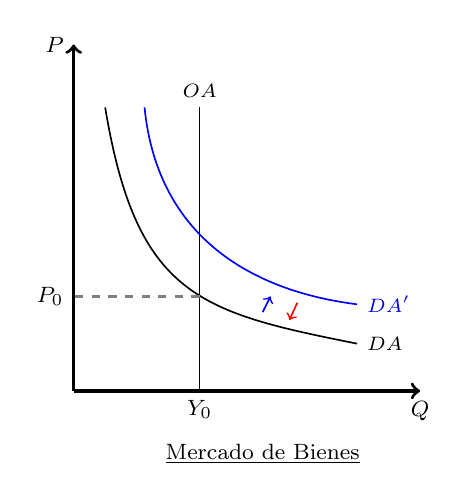
\begin{tikzpicture}[scale=0.4]
\draw[very thick,<-] (0,11)--(0,0);
\draw[very thick,->] (0,0)--(11,0) node[below]{\footnotesize $Q$};
\node[left] at (0,11) {\footnotesize $P$};

\node[] at(6,-2) {\footnotesize \underline{Mercado de Bienes}};
\draw[semithick] (1,9).. controls (2,3) and (4, 2.5) .. (9, 1.5) node [right]{\scriptsize $DA$};
\draw[semithick](4, 0)--(4, 9) node [above]{\scriptsize $OA$};
\draw[thick, gray, dashed] (4,3)--(0,3) node [left, black]{\footnotesize $P_0$};
\node[below] at(4,0) {\footnotesize $Y_0$};
\draw[semithick, blue] (2.25,9).. controls (2.75,4) and (7, 3) .. (9, 2.75) node [right]{\scriptsize $DA'$};
\draw[semithick, ->, blue] (6,2.5)--(6.25,3);
\only<2->{
\draw[semithick, <-, red] (6.85,2.25)--(7.1,2.8);
}
\end{tikzpicture}
\end{center}
     \end{minipage}
  %  \hfill
    \begin{minipage}[b]{0.45\textwidth}
    \begin{center}
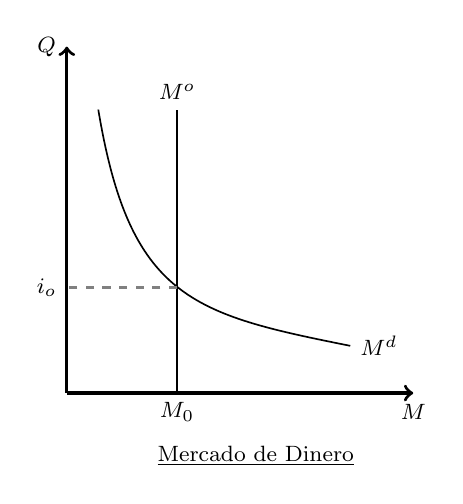
\begin{tikzpicture}[scale=0.4]
\draw[very thick,<-] (0,11) node[left]{\footnotesize $Q$}--(0,0);
\draw[very thick,->] (0,0)--(11,0) node[below]{\footnotesize $M$};
\node[below] at (3.5, 0) {\footnotesize $M_{0}$};

\node[] at(6,-2) {\footnotesize \underline{Mercado de Dinero}};
\draw[semithick] (1,9).. controls (2,3) and (4, 2.5) .. (9, 1.5) node [right]{\footnotesize $M^{d}$};
\draw[semithick](3.5, 0)--(3.5, 9) node [above]{\footnotesize $M^{o}$};
 \draw[thick, gray, dashed] (3.5,3.35)--(0,3.35) node [left, black]{\footnotesize $i_{o}$};
\end{tikzpicture}
\end{center}
    \end{minipage}
\end{center}
\end{figure}
\end{center}   
\begin{itemize}
\footnotesize
    \item Aumenta la $DA$: $DA'= C+ I+ \textcolor{blue}{\uparrow G } $.
    \only<2->{
    \item Pero el consumo privado cae en la misma proporción que el gasto, porque el ingreso disponible cae permanentemente: $DA= \textcolor{red}{\downarrow C }+ I+ \uparrow G $.
    \item Hay solo un cambio en la composición de la DA.}
\end{itemize}
\end{frame}

\begin{frame}{Expansión fiscal con impuestos permanentes (keynesiano)}
\begin{center}
\begin{figure}[H]
\begin{center}
    \begin{minipage}[b]{0.45\textwidth}
        \begin{center}
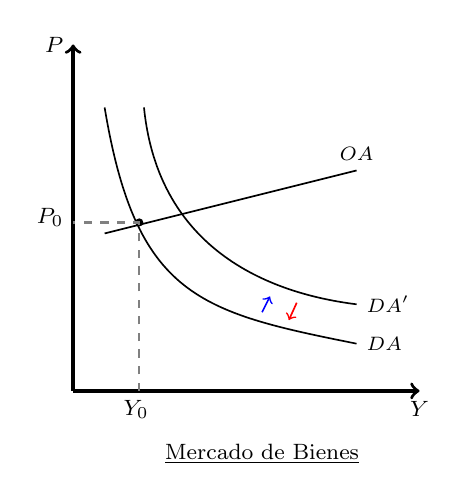
\begin{tikzpicture}[scale=0.4]
\draw[very thick,<-] (0,11)--(0,0);
\draw[very thick,->] (0,0)--(11,0) node[below]{\footnotesize $Y$};
\node[left] at (0,11) {\footnotesize $P$};
\node[] at(6,-2) {\footnotesize \underline{Mercado de Bienes}};
\draw[semithick] (1,9).. controls (2,3) and (4, 2.5) .. (9, 1.5) node [right]{\scriptsize $DA$};
\draw[semithick] (2.25,9).. controls (2.75,4) and (7, 3) .. (9, 2.75) node [right]{\scriptsize $DA'$};
\draw[semithick](1, 5)--(9,7) node [above]{\scriptsize $OA$};
\draw[semithick, ->, blue] (6,2.5)--(6.25,3);
\draw[semithick, <-, red] (6.85,2.25)--(7.1,2.8);
\node[below] at (2,0) {\footnotesize $Y_0$};
\node[left] at (0,5.5) {\footnotesize $P_0$};
\draw[fill] (2.1,5.35) circle [radius =0.11];
 \draw[thick, gray, dashed] (2.1,0)--(2.1,5.35)--(0,5.35);

\end{tikzpicture}
\end{center}
     \end{minipage}
  %  \hfill
    \begin{minipage}[b]{0.45\textwidth}
    \begin{center}
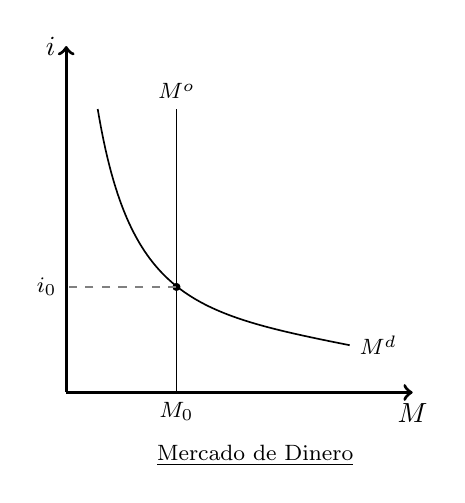
\begin{tikzpicture}[scale=0.4]
\draw[very thick,<-] (0,11) node[left]{$i$}--(0,0);
\draw[very thick,->] (0,0)--(11,0) node[below]{$M$};
\node[right] at (0,11) {};

\node[] at(6,-2) {\footnotesize \underline{Mercado de Dinero}};
\draw[semithick] (1,9).. controls (2,3) and (4, 2.5) .. (9, 1.5) node [right]{\footnotesize $M^{d}$};
\draw[semithick](3.5, 0)--(3.5, 9) node [above]{\footnotesize $M^{o}$};
\node[below] at (3.5,0) {\footnotesize $M_0$};
\node[left] at (0,3.35) {\footnotesize $i_0$};
\draw[fill] (3.5,3.35) circle [radius =0.11];
\draw[thick, gray, dashed] (3.5,3.35)--(0,3.35);

\end{tikzpicture}
\end{center}
    \end{minipage}
\end{center}
\end{figure}
\end{center} 

\begin{itemize}
\footnotesize
    \item El resultado es igual que en el mundo clásico: lo que gasta demás el Estado lo gasta de menos la gente: $DA = \textcolor{red}{\downarrow C }+ I+ \textcolor{blue}{\uparrow G } $.
\end{itemize}
\end{frame}

\begin{frame}{Expansión fiscal con impuestos \textbf{transitorios}}
   \begin{itemize}
       \item El consumo no disminuye por el monto total del impuesto dado que esta situación es transitoria (en el próximo período el individuo vuelve a tener su ingreso total)
       \item Los agentes elegirán endeudarse para suavizar la caída del ingreso por el impuesto. 
       \item El proceso depende del enfoque que usemos:
        \begin{itemize}
        \item  En el mundo clásico, el aumento transitorio del gasto financiado con impuestos no afecta el producto por el \textit{crowding out} total
        \item En el mundo keynesiano, el producto se expande transitoriamente, pero al retirarse el gasto y con precios más altos, la economía entra en recesión antes de volver al equilibrio.
        \end{itemize}
   \end{itemize}
\end{frame}


\begin{frame}{Expansión fiscal con impuestos transitorios (clásico)}
\begin{center}
\begin{figure}[H]
\begin{center}
    \begin{minipage}[b]{0.4\textwidth}
        \begin{center}
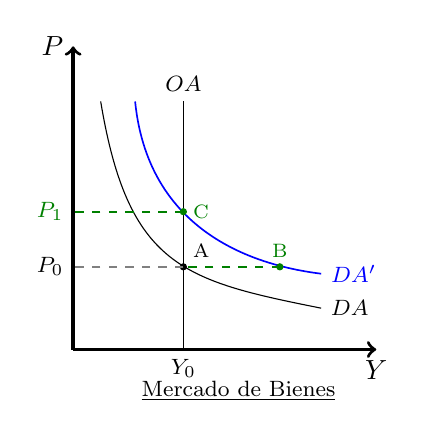
\begin{tikzpicture}[scale=0.35]
\draw[very thick,<-] (0,11)--(0,0);
\draw[very thick,->] (0,0)--(11,0) node[below]{$Y$};
\node[left] at (0,11) {$P$};
\node[] at(6,-1.5) {\footnotesize \underline{Mercado de Bienes}};
\draw[thin] (1,9).. controls (2,3) and (4, 2.5) .. (9, 1.5) node [right]{\footnotesize $DA$};
\node[below] at (4,0) {\footnotesize $Y_0$};
\node[left] at (0,3) {\footnotesize $P_0$};
\draw[fill] (4,3) circle [radius =0.11] circle [radius =0.11] node[above right] {\scriptsize A};
\draw[thin](4, 0)--(4, 9) node [above]{\footnotesize $OA$};
\draw[semithick, blue] (2.25,9).. controls (2.75,4) and (7, 3) .. (9, 2.75) node [right]{\footnotesize $DA'$};
\draw[thick, gray, dashed] (4,3)--(0,3);
\only<2->{
\draw[fill, green!50!black] (7.5,3) circle [radius =0.11] node[above] {\scriptsize B};
\draw[thick, green!50!black, dashed] (7.5,3)--(4,3);

\draw[thick, green!50!black, dashed] (4,5)--(0,5);
\draw[fill, green!50!black] (4,5) circle [radius =0.11] node[right] {\scriptsize C};
\node[left, green!50!black] at (0,5) {\footnotesize $P_1$};
}
%\draw[thick, gray, dashed] (2.1,0)--(2.1,5.35)--(0,5.35);
\end{tikzpicture}
\end{center}
     \end{minipage}
  %  \hfill
    \begin{minipage}[b]{0.4\textwidth}
    \begin{center}
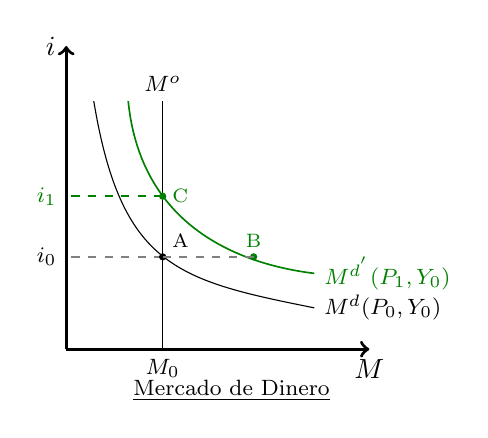
\begin{tikzpicture}[scale=0.35]
\draw[very thick,<-] (0,11) node[left]{$i$}--(0,0);
\draw[very thick,->] (0,0)--(11,0) node[below]{$M$};
\node[right] at (0,11) {};
\node[] at(6,-1.5) {\footnotesize \underline{Mercado de Dinero}};
\draw[thin] (1,9).. controls (2,3) and (4, 2.5) .. (9, 1.5) node [right]{\footnotesize $M^{d} (P_0, Y_0)$};
\draw[thin](3.5, 0)--(3.5, 9) node [above]{\footnotesize $M^{o}$};
\node[below] at (3.5,0) {\footnotesize $M_0$};
\node[left] at (0,3.35) {\footnotesize $i_0$};
 \draw[thick, gray, dashed] (3.5,3.35)--(0,3.35);
\draw[fill] (3.5,3.35) circle [radius =0.11] node[above right] {\scriptsize A};

\only<2->{
\draw[semithick, green!50!black] (2.25,9).. controls (2.75,4) and (7, 3) .. (9, 2.75) node [right]{\footnotesize $M^{d^{'}} (P_1, Y_0)$};
\draw[fill, green!50!black] (6.8,3.35) circle [radius =0.11] node[above] {\scriptsize B};
\draw[thick, gray, dashed] (6.8,3.35)--(3.5,3.35);
\draw[fill, green!50!black] (3.5,5.55) circle [radius =0.11] node[right] {\scriptsize C};
\node[left, green!50!black] at (0,5.55) {\footnotesize $i_1$};
 \draw[thick, green!50!black, dashed] (3.5,5.55)--(0,5.55);
}


\end{tikzpicture}
\end{center}
    \end{minipage}
\end{center}
\end{figure}
\end{center} 
    \begin{itemize}
        \scriptsize
        \item Aumenta la $DA$: $DA'=$ \textcolor{blue}{ $\downarrow C$} $+ I+$ \textcolor{blue}{$\uparrow \uparrow G $} $\rightarrow$ Se genera un exceso de demanda (punto B) que presiona los precios hacia arriba.
        \only<2->{
            \item \textcolor{green!50!black}{A medida que suben los precios la demanda de dinero aumenta y también la tasa de interés. $\rightarrow$ En el mercado de credito, la oferta de FP se desplaza hacia la izquierda produciendo el crowding out.} 
        }
        \only<3->{\item Este crowding out es total, por lo que la DA vuelve a sus cantidades originales (punto C) y el producto no se mueve $\rightarrow$ Cuando la política fiscal se revierte tenes una pequeña etapa de recesión.}
    \end{itemize}
\end{frame}


\begin{frame}{Expansión fiscal con impuestos transitorios (keynesiano)}
\begin{center}
\begin{figure}[H]
\renewcommand{\figurename}{Figure}
\begin{center}
    \begin{minipage}[b]{0.4\textwidth}
        \begin{center}
\begin{tikzpicture}[scale=0.35]
\draw[very thick,<-] (0,11)--(0,0);
\draw[very thick,->] (0,0)--(11,0) node[below]{$Y$};
\node[left] at (0,11) {$P$};

\node[] at(6,-2.5) {\footnotesize \underline{Mercado de Bienes}};
\draw[thin] (1,9).. controls (2,3) and (4, 2.5) .. (9, 1.5) node [right]{\scriptsize $DA$};
\draw[thin](0, 5)--(9, 7) node [right]{\scriptsize $OA$};
\draw [thin,decorate,decoration={brace,amplitude=3pt, mirror},xshift=5pt,yshift=0pt](2.1,-1.25) -- (5.3,-1.25);
\draw (4,-1.75) node[]{\scriptsize $\Delta G $};
\draw[thick, gray, dashed] (2.1,5.5)--(0,5.5);
\draw[fill] (2.1,5.5) circle [radius =0.11] node[below left] {\scriptsize $A$}; 
\node[below] at (2.1,0) {\scriptsize $Y_0$};
\node[left] at (0,5.2) {\scriptsize $P_0$};
\draw[fill, blue] (2.8,5.65) circle [radius =0.11] node[above right] {\scriptsize $B$}; 
\draw[thin, blue] (1.75,9).. controls (2.25,3.5) and (6.5,2.5) .. (9, 2.25) node [right]{\scriptsize $DA'$};
\node[left, blue] at (0,5.75) {\scriptsize $P_1$};
\node[below, blue] at (2.8,0) {\scriptsize $Y_1$};
\draw[thick, blue, dashed] (2.8,0)--(2.8,5.65)--(0,5.65);
\draw[thick, gray, dashed] (5.5,6.3)--(5.5,0);
\only<2->{
    \draw[fill, green!50!black] (2.1,6.8) circle [radius =0.11] node[right] {\scriptsize $C$}; 
    \draw[thick, green!50!black] (2.1,0)--(2.1,9) node [right]{\scriptsize $OALP$};
}
\only<3->{
    
    \draw[semithick, red] (1,9).. controls (2,3) and (4, 2.5) .. (9, 1.5) node [right]{\scriptsize $DA$};
    \draw[fill, red] (1.45,6.8) circle [radius =0.11] node[above left] {\scriptsize $D$}; 
    \node[left, red] at (0,6.8) {\scriptsize $P_2$};
     \draw[thick, red, dashed] (2.1,6.8)--(0,6.8);
}

\end{tikzpicture}
\end{center}
     \end{minipage}
  %  \hfill
    \begin{minipage}[b]{0.4\textwidth}
    \begin{center}
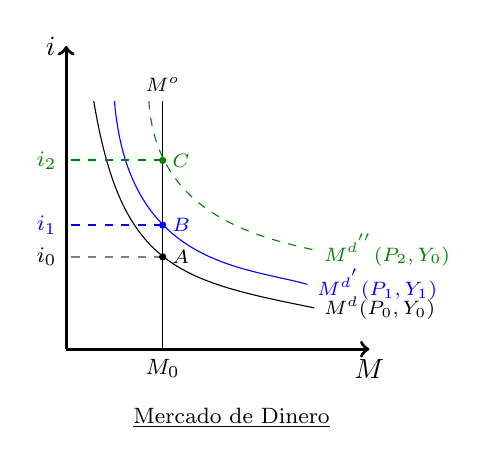
\begin{tikzpicture}[scale=0.35]
\draw[very thick,<-] (0,11) node[left]{$i$}--(0,0);
\draw[very thick,->] (0,0)--(11,0) node[below]{$M$};
\node[right] at (0,11) {};
\node[] at(6,-2.5) {\footnotesize \underline{Mercado de Dinero}};
\draw[thin] (1,9).. controls (2,3) and (4, 2.5) .. (9, 1.5) node [right]{\scriptsize $M^{d} (P_0, Y_0)$};
\node[below] at (3.5,0) {\footnotesize $M_0$};
\node[left] at (0,3.35) {\footnotesize $i_0$};
\draw[thin](3.5, 0)--(3.5, 9) node [above]{\scriptsize $M^{o}$};
\draw[thick, gray, dashed] (3.5,3.35)--(0,3.35);
\draw[thick, blue, dashed] (3.5,4.5)--(0,4.5);
\draw[fill] (3.5,3.35) circle [radius =0.11] node[right] {\scriptsize $A$}; 
\draw[thin, blue] (1.75,9).. controls (2.25,3) and (6.5, 3) .. (8.75, 2.35) node [right]{\scriptsize $M^{d^{'}} (P_1, Y_1)$};
\draw[fill, blue] (3.5,4.5) circle [radius =0.11] node[right] {\scriptsize $B$}; 
\node[left, blue] at (0,4.5) {\footnotesize $i_1$};

\only<2->{
    \draw[fill, green!50!black] (3.5,6.85) circle [radius =0.11] node[right] {\scriptsize $C$};
    \draw[thin, green!50!black, dashed] (3,9).. controls (3.25,5) and (6.75,4.1) .. (9,3.6) node [right]{\scriptsize $M^{d^{''}} (P_2, Y_0)$};
    \draw[thick, green!50!black, dashed] (3.5,6.85)--(0,6.85);
    \node[left, green!50!black] at (0,6.85) {\footnotesize $i_2$};
}
\end{tikzpicture}
\end{center}
    \end{minipage}
\end{center}
\end{figure}
\end{center}
    \begin{itemize}
        \scriptsize
        \item \textcolor{blue}{Aumenta la $DA$ ($DA'= \downarrow C + I + \uparrow \uparrow G $) y la demanda de dinero sube} $\rightarrow$ la tasa de interés sube menos que en el caso clásico ya que el producto se expande.
        \only<2->{
            \item En el LP estamos encima del pleno empleo, \textcolor{green!50!black}{los precios empiezan a subir y el efecto expansivo se reduce hasta C, aumentando a la vez la demanda de dinero}
        }
        \only<3->{ \item Cuando el gasto público cae, \textcolor{red}{$DA$ vuelve a su original en el punto D (recesión)}. El exceso de oferta en $P_2$ genera una presión deflacionaria hasta llegar a A}
    \end{itemize}
\end{frame}

\begin{frame}{Expansión fiscal financiada con deuda}
   \begin{itemize}
        \item Acá el punto clave es si los agentes anticipan la carga impositiva que implica la mayor deuda
        \begin{itemize}
            \item Si los agentes anticipan que el gobierno va a tener que subir impuestos en el futuro para pagar la deuda, entonces el efecto es el mismo que si se financiara con impuestos.
            \begin{itemize}
                \item En este caso decimos que los agentes son \textbf{ricardianos}.
            \end{itemize}
            \item Si los agentes no anticipan la carga impositiva, entonces el efecto es distinto.
            \begin{itemize}
                \item En este caso decimos que los agentes son \textbf{no ricardianos}.
            \end{itemize}
        \end{itemize}
        \item En la práctica se encuentra que el ahorro responde a la deuda, pero que la compensación no es plena.
        \item En tanto el efecto no es de compensación plena, hay un efecto expansivo en la demanda agregada (con efecto sobre el producto en un mundo keynesiano).
    \end{itemize}
\end{frame}

\begin{frame}{Ejemplo de equivalencia ricardiana}
    \begin{itemize}
        \item Supongamos dos periodos en los que el individuo tiene ingresos de 1000 y 1000
        \item El gobierno quiere gastar 100 y 100 
        \item Lo financia con deuda en el primer periodo y la tasa de interés es 10\%
        \item El agente enfrenta impuestos de 0 y 210
        \item Si consume su ingreso consumiría 1000 y 790 
        \item ¿Qué pasa si ahorra 100 en el primero período?
        \item Ahora puede consumir 900 y 900 (que es mejor que 1000 y 790)
        \item Pero 900 y 900 ¡es lo mismo que si el gobierno hubiera financiado los 100 con impuestos! 
    \end{itemize}
\end{frame}

\begin{frame}{¿Pero existe ese fenómeno Ricardiano? I}
    \begin{center}
        Correlación entre deuda pública y activos financieros netos acumulados por los hogares
    \end{center}
    \centering\includegraphics[width=11cm]{../Figures/C41.6.png}\  
\end{frame}

\begin{frame}{Expansión fiscal permanente financiada con deuda y agentes ricardianos}
    \begin{center}
    \begin{figure}[H]
    \begin{center}
    \begin{minipage}[b]{0.4\textwidth}
    \begin{center}
    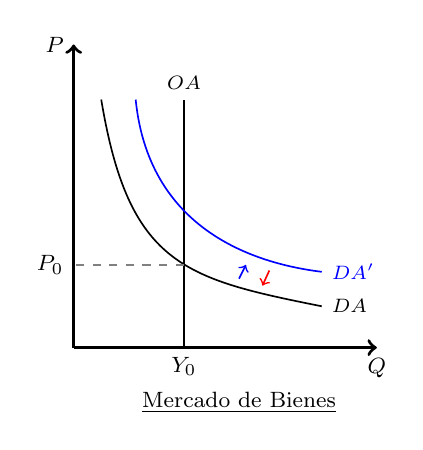
\begin{tikzpicture}[scale=0.35]
    \draw[very thick,<-] (0,11)--(0,0);
    \draw[very thick,->] (0,0)--(11,0) node[below]{\footnotesize $Q$};
    \node[left] at (0,11) {\footnotesize $P$};

    \node[] at(6,-2) {\footnotesize \underline{Mercado de Bienes}};
    \draw[semithick] (1,9).. controls (2,3) and (4, 2.5) .. (9, 1.5) node [right]{\scriptsize $DA$};
    \draw[semithick](4, 0)--(4, 9) node [above]{\scriptsize $OA$};
    \draw[thick, gray, dashed] (4,3)--(0,3) node [left, black]{\footnotesize $P_0$};
    \node[below] at(4,0) {\footnotesize $Y_0$};
    \draw[semithick, blue] (2.25,9).. controls (2.75,4) and (7, 3) .. (9, 2.75) node [right]{\scriptsize $DA'$};
    \draw[semithick, ->, blue] (6,2.5)--(6.25,3);
    \only<2->{
    \draw[semithick, <-, red] (6.85,2.25)--(7.1,2.8);
    }
    \end{tikzpicture}
    \end{center}
        \end{minipage}
    %  \hfill
        \begin{minipage}[b]{0.4\textwidth}
        \begin{center}
    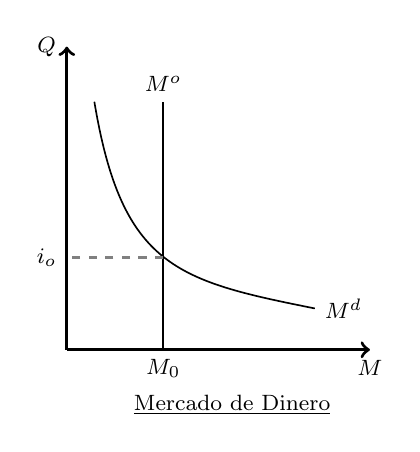
\begin{tikzpicture}[scale=0.35]
    \draw[very thick,<-] (0,11) node[left]{\footnotesize $Q$}--(0,0);
    \draw[very thick,->] (0,0)--(11,0) node[below]{\footnotesize $M$};
    \node[below] at (3.5, 0) {\footnotesize $M_{0}$};

    \node[] at(6,-2) {\footnotesize \underline{Mercado de Dinero}};
    \draw[semithick] (1,9).. controls (2,3) and (4, 2.5) .. (9, 1.5) node [right]{\footnotesize $M^{d}$};
    \draw[semithick](3.5, 0)--(3.5, 9) node [above]{\footnotesize $M^{o}$};
    \draw[thick, gray, dashed] (3.5,3.35)--(0,3.35) node [left, black]{\footnotesize $i_{o}$};
    \end{tikzpicture}
    \end{center}
        \end{minipage}
    \end{center}
    \end{figure}
    \end{center}   
    \begin{itemize}
        \scriptsize
        \item Aumenta la $DA$: $DA'= C+ I+ \textcolor{blue}{\uparrow G } $.
        \only<2->{
        \item Pero el consumo privado cae en la misma proporción que el gasto, porque aumenta el ahorro: $DA= \textcolor{red}{\downarrow C}+ I+ \uparrow G $.
        \item El gobierno aumenta la deuda y desplaza la demanda de crédito pero también aumenta la oferta de crédito porque aumenta el ahorro.
        \item El efecto es igual en el caso clásico y en el keynesiano.
        }
    \end{itemize}
\end{frame}

\begin{frame}{Expansión fiscal transitoria financiada con deuda y agentesricardianos}
    \begin{itemize}
        \item En resumen, si el gasto público es permanente y se financia con deuda tenemos el mismo efecto que si se financia con impuestos, ya que los agentes anticipan el aumento de impuestos futuros. Ahora bien, el mecanismo es distinto: aumentan la oferta de FP y la demanda de FP.
        \item Si el aumento del gasto público es transitorio y financiado con deuda
        \begin{itemize}
            \item La demanda agregada se incrementa de la misma manera que cuando el aumento del gasto es transitorio, pero
            financiado a través de impuestos.
            \item Se produce la misma expansión en la demanda de crédito, pero es el gobierno quien lo causa, mientras que los individuos modifican muy poco su nivel de consumo.
        \end{itemize}
    \end{itemize}
\end{frame}

\begin{frame}{Expansión fiscal transitoria financiada con deuda y agentes no ricardianos (clásico)}
\begin{center}
\begin{figure}[H]
\begin{center}
    \begin{minipage}[b]{0.4\textwidth}
        \begin{center}
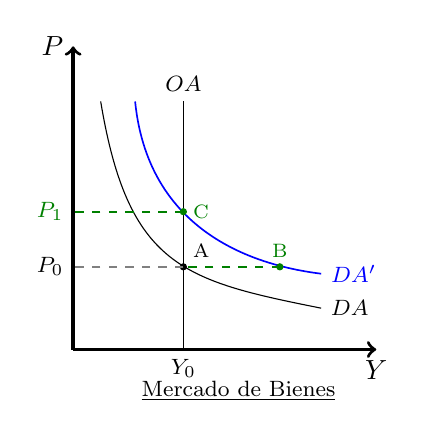
\begin{tikzpicture}[scale=0.35]
\draw[very thick,<-] (0,11)--(0,0);
\draw[very thick,->] (0,0)--(11,0) node[below]{$Y$};
\node[left] at (0,11) {$P$};
\node[] at(6,-1.5) {\footnotesize \underline{Mercado de Bienes}};
\draw[thin] (1,9).. controls (2,3) and (4, 2.5) .. (9, 1.5) node [right]{\footnotesize $DA$};
\node[below] at (4,0) {\footnotesize $Y_0$};
\node[left] at (0,3) {\footnotesize $P_0$};
\draw[fill] (4,3) circle [radius =0.11] circle [radius =0.11] node[above right] {\scriptsize A};
\draw[thin](4, 0)--(4, 9) node [above]{\footnotesize $OA$};
\draw[semithick, blue] (2.25,9).. controls (2.75,4) and (7, 3) .. (9, 2.75) node [right]{\footnotesize $DA'$};
\draw[thick, gray, dashed] (4,3)--(0,3);
\only<2->{
\draw[fill, green!50!black] (7.5,3) circle [radius =0.11] node[above] {\scriptsize B};
\draw[thick, green!50!black, dashed] (7.5,3)--(4,3);

\draw[thick, green!50!black, dashed] (4,5)--(0,5);
\draw[fill, green!50!black] (4,5) circle [radius =0.11] node[right] {\scriptsize C};
\node[left, green!50!black] at (0,5) {\footnotesize $P_1$};
}
%\draw[thick, gray, dashed] (2.1,0)--(2.1,5.35)--(0,5.35);
\end{tikzpicture}
\end{center}
     \end{minipage}
  %  \hfill
    \begin{minipage}[b]{0.4\textwidth}
    \begin{center}
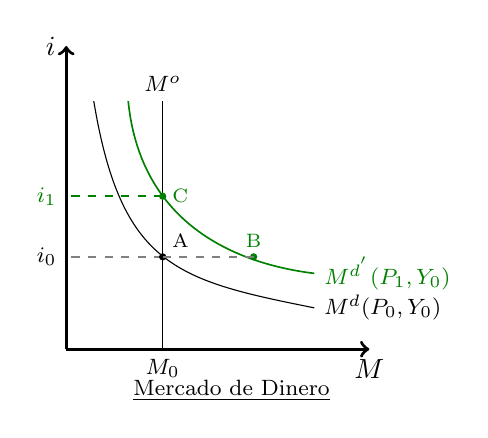
\begin{tikzpicture}[scale=0.35]
\draw[very thick,<-] (0,11) node[left]{$i$}--(0,0);
\draw[very thick,->] (0,0)--(11,0) node[below]{$M$};
\node[right] at (0,11) {};
\node[] at(6,-1.5) {\footnotesize \underline{Mercado de Dinero}};
\draw[thin] (1,9).. controls (2,3) and (4, 2.5) .. (9, 1.5) node [right]{\footnotesize $M^{d} (P_0, Y_0)$};
\draw[thin](3.5, 0)--(3.5, 9) node [above]{\footnotesize $M^{o}$};
\node[below] at (3.5,0) {\footnotesize $M_0$};
\node[left] at (0,3.35) {\footnotesize $i_0$};
 \draw[thick, gray, dashed] (3.5,3.35)--(0,3.35);
\draw[fill] (3.5,3.35) circle [radius =0.11] node[above right] {\scriptsize A};

\only<2->{
\draw[semithick, green!50!black] (2.25,9).. controls (2.75,4) and (7, 3) .. (9, 2.75) node [right]{\footnotesize $M^{d^{'}} (P_1, Y_0)$};
\draw[fill, green!50!black] (6.8,3.35) circle [radius =0.11] node[above] {\scriptsize B};
\draw[thick, gray, dashed] (6.8,3.35)--(3.5,3.35);
\draw[fill, green!50!black] (3.5,5.55) circle [radius =0.11] node[right] {\scriptsize C};
\node[left, green!50!black] at (0,5.55) {\footnotesize $i_1$};
 \draw[thick, green!50!black, dashed] (3.5,5.55)--(0,5.55);
}


\end{tikzpicture}
\end{center}
    \end{minipage}
\end{center}
\end{figure}
\end{center} 
    \begin{itemize}
        \scriptsize
        \item Aumenta la $DA$: $DA'=$ \textcolor{blue}{ $\downarrow C$} $+ I+$ \textcolor{blue}{$\uparrow \uparrow G $} $\rightarrow$ Ya que los agentes no internalizan los mayores impuestos futuros.
        \only<2->{
            \item \textcolor{green!50!black}{A medida que suben los precios la demanda de dinero aumenta y también la tasa de interés. $\rightarrow$ En el mercado de credito, la demanda de FP se desplaza hacia la derecha produciendo el crowding out.} 
        }
        \only<3->{\item Este crowding out es total y los resultados terminan siendo iguales a los otros aumentos transitorios en el gasto.}
    \end{itemize}
\end{frame}


\begin{frame}{Expansión fiscal financiada con deuda y agentes no ricardianos (keynesiano)}
    \begin{center}
        \begin{figure}[H]
        \renewcommand{\figurename}{Figure}
        \begin{center}
        \begin{minipage}[b]{0.4\textwidth}
        \begin{center}
        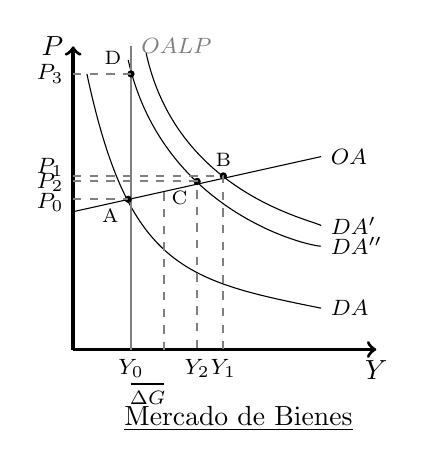
\begin{tikzpicture}[scale=0.35]
        \draw[very thick,<-] (0,11)--(0,0);
        \draw[very thick,->] (0,0)--(11,0) node[below]{$Y$};
        \node[left] at (0,11) {$P$};
        \node[] at(6,-2.5) {\underline{Mercado de Bienes}};
        \draw[thin] (0.5,10).. controls (2,3) and (4, 2.5) .. (9, 1.5) node [right]{\footnotesize $DA$};
        \draw[thin] (2.65,10.75).. controls (3.75,5.75) and (8.5, 4.75) .. (9, 4.5) node [right]{\footnotesize $DA'$};
        \draw[thin] (2,10.5).. controls (3.25,5) and (8.5, 3.75) .. (9, 3.75) node [right]{\footnotesize $DA''$};
        \draw[thin](0, 5)--(9, 7) node [right]{\footnotesize $OA$};
        \draw [thin](2.1,-1.25) -- (3.3,-1.25);
        \draw (2.7,-1.75) node[]{\scriptsize $\Delta G $};
        \draw[thick, gray] (2.1,0)--(2.1,11) node [right]{\footnotesize $OALP$};
        \draw[thick, gray, dashed] (3.3,5.7)--(3.3,0); 
        \draw[fill] (2,5.45) circle [radius =0.11] node[below left] {\scriptsize A};  
        \draw[fill] (5.45,6.3) circle [radius =0.11] node[above] {\scriptsize B}; 
        \draw[fill] (4.5,6.1) circle [radius =0.11] node[below left] {\scriptsize C};  
        \draw[fill] (2.1,10) circle [radius =0.11] node[above left] {\scriptsize D};  
        \node[below] at (2.1,0) {\footnotesize $Y_0$};
        \node[below] at (5.45,0) {\footnotesize $Y_1$};
        \node[below] at (4.5,0) {\footnotesize $Y_2$};
        \node[left] at (0,5.35) {\footnotesize $P_0$};
        \node[left] at (0,6.6) {\footnotesize $P_1$};
        \node[left] at (0,6.05) {\footnotesize $P_2$};
        \node[left] at (0,10) {\footnotesize $P_3$};
        \draw[thick, gray, dashed] (0,5.45)--(2,5.45);
        \draw[thick, gray, dashed] (0,6.3)--(5.45,6.3)--(5.45,0);
        \draw[thick, gray, dashed] (0,6.1)--(4.5,6.1)--(4.5,0);
        \draw[thick, gray, dashed] (0,10)--(2.1,10);
        \end{tikzpicture}
        \end{center}
        \end{minipage}
        \begin{minipage}[b]{0.4\textwidth}
        \begin{center}
        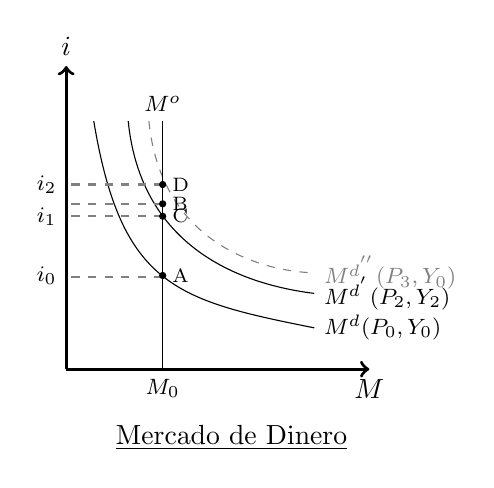
\begin{tikzpicture}[scale=0.35]
        \draw[very thick,<-] (0,11) node[above]{$i$}--(0,0);
        \draw[very thick,->] (0,0)--(11,0) node[below]{$M$};
        \node[right] at (0,11) {};
        \node[] at(6,-2.5) {\underline{Mercado de Dinero}};
        \draw[thin] (1,9).. controls (2,3) and (4, 2.5) .. (9, 1.5) node [right]{\footnotesize $M^{d} (P_0, Y_0)$};
        \draw[thin] (2.25,9).. controls (2.75,4) and (7, 3) .. (9, 2.75) node [right]{\footnotesize $M^{d^{'}} (P_2, Y_2)$};
        \draw[thin, gray, dashed] (3,9).. controls (3.5,4) and (8, 3.5) .. (9,3.5) node [right]{\footnotesize $M^{d^{''}} (P_3, Y_0)$};
        \draw[thin](3.5, 0)--(3.5, 9) node [above]{\footnotesize $M^{o}$};
        \draw[thick, gray, dashed] (3.5,3.35)--(0,3.35);
        \draw[thick, gray, dashed] (3.5,5.55)--(0,5.55);
        \draw[thick, gray, dashed] (3.5,6)--(0,6);
        \draw[thick, gray, dashed] (3.5,6.7)--(0,6.7);
        \draw[fill] (3.5,3.4) circle [radius =0.11] node[right] {\scriptsize A};
        \draw[fill] (3.5,5.55) circle [radius =0.11] node[right] {\scriptsize C};  
        \draw[fill] (3.5,6) circle [radius =0.11] node[right] {\scriptsize B};  
        \draw[fill] (3.5,6.7) circle [radius =0.11] node[right] {\scriptsize D}; 
        \node[below] at (3.5,0) {\footnotesize $M_0$};
        \node[left] at (0,3.4) {\footnotesize $i_0$};
        \node[left] at (0,5.55) {\footnotesize $i_1$};
        \node[left] at (0,6.7) {\footnotesize $i_2$};
        \end{tikzpicture}
        \end{center}
        \end{minipage}
        \end{center}
        \end{figure}
    \end{center}
    \begin{itemize}
        \scriptsize
        \item Aumenta la $DA$ y al aumentar el producto eso produce un \textbf{efecto multiplicador} vía un mayor consumo: $DA'=$ \textcolor{blue}{ $\uparrow C$} $+ I+$ \textcolor{blue}{$\uparrow \uparrow G $}
        \only<2->{
            \item \textcolor{green!50!black}{La expansion del producto y los precios eleva la demanda de dinero y, por ende, la tasa de interés. Si bien sube la tasa de interés, el efecto multiplicador prima por ende hay expansión del producto.} 
        }
        \only<3->{\item A largo plazo, el crowding out se termina produciendo y debemos volver a un equilibrio en el producto de LP.}
    \end{itemize}
\end{frame}

\begin{frame}{Discusión}

    \begin{itemize}
    \item Para un clásico hay poco por hacer: más vale concentrarte en lo estructural (competencia, apertura, instituciones).
    \item En el mundo keynesiano, al menos hay margen, pero…
    \item A) La mayor parte de los cambios en el producto son generados por cambios en C e I, causados por los agentes individuales, inducidos por el ambiente político y las expectativas
    \item B) ¿Estamos seguros el gobierno será efectivo o incluso si actuará cuando debe actuar? 
    \end{itemize}

\end{frame}

\begin{frame}{Caveats a la política macroeconómica}
    \begin{itemize}
    \item Puede existir un problema de rezagos: las políticas pueden hacerse en un momento inadecuado
    \item Podes pensar que podes cuando no podes (si el mundo es clásico, las políticas sólo van a resultar en inflación o deflación)
    \item Si el marco político genera gobiernos débiles, puede existir prociclicalidad fiscal o exceso de gasto
    \item Las políticas pueden incrementar la incertidumbre y las expectativas son \textbf{fundamentales}.
    \item La gente puede anticipar estas políticas haciéndolas menos efectivas (inconsistencia temporal y expectativas racionales), por ejemplo si vos aumentas el dinero y la gente se da cuenta al toque, los precios suben y no lográs nada
    \end{itemize}
\end{frame}

% \begin{frame}{Los casos de Política Fiscal}

% \centering
% \scalebox{0.75}{
% \begin{tikzpicture}[
%   node distance=0.5cm and 0.9cm,
%   every node/.style={font=\footnotesize},
%   box/.style={rectangle, rounded corners, draw=blue!50, fill=blue!10, align=center, minimum width=2cm, minimum height=1cm},
%   resultA/.style={rectangle, draw=black, fill=green!10, align=center, minimum width=2cm, minimum height=1cm},
%     resultB/.style={rectangle, draw=black, fill=red!10, align=center, minimum width=2cm, minimum height=1cm},
%     resultC/.style={rectangle, draw=black, fill=yellow!10, align=center, minimum width=2cm, minimum height=1cm},
%   arrow/.style={thick, ->, >=stealth}
%   ]
% % Nivel 1
% \node[box] (start) {\textbf{Aumento del} \\ \textbf{Gasto Público}};

% % Nivel 2
% \node[box, below left=of start, xshift=-1cm] (imp) {Financiado con \\ \textbf{Impuestos}};
% \node[box, below right=of start, xshift=1cm] (deuda) {Financiado con \\ \textbf{Deuda}};

% % Nivel 3 impuestos
% \node[box, below=of imp, xshift=-1.5cm] (imp_perm) {Permanente};
% \node[box, below=of imp, xshift=1.5cm] (imp_trans) {Transitorio$^\textbf{*}$};

% % Resultados impuestos
% \node[resultA, below=of imp_perm] (r1) {DA no cambia\\(↑G = ↓C)};
% \node[resultB, below=of imp_trans] (r2) {↑DA temporalmente\\ (↑G $>$ ↓C )};

% % Nivel 3 deuda
% \node[box, below=of deuda, xshift=-2cm] (ric) {Agentes\\ Ricardianos};
% \node[box, below=of deuda, xshift=2cm] (noric) {Agentes\\ No Ricardianos$^\textbf{*}$};

% % Subniveles ricardianos
% \node[box, below=of ric, xshift=-1.5cm] (ric_perm) {Permanente};
% \node[box, below=of ric, xshift=1.5cm] (ric_trans) {Transitorio$^\textbf{*}$};

% \node[resultA, below=of ric_perm] (r3) {DA no cambia\\(↑G = ↓C)};
% \node[resultB, below=of ric_trans] (r4) {↑DA temporalmente\\ (↑G $>$ ↓C )};

% % Subniveles no ricardianos
% %\node[result, below=of noric, xshift=-2cm] (r5) {DA ↑ fuerte\\(Multiplicador ↑)};
% \node[resultC, below=of noric, xshift=1.2cm] (r6) {↑DA \\ \underline{Clásicos}: ↑DA$=$↑G \\ \underline{Keynesianos}: ↑DA$>$↑G \\(multiplicador)};

% % Flechas
% \draw[arrow] (start) -- (imp);
% \draw[arrow] (start) -- (deuda);

% \draw[arrow] (imp) -- (imp_perm);
% \draw[arrow] (imp) -- (imp_trans);
% \draw[arrow] (imp_perm) -- (r1);
% \draw[arrow] (imp_trans) -- (r2);

% \draw[arrow] (deuda) -- (ric);
% \draw[arrow] (deuda) -- (noric);
% \draw[arrow] (ric) -- (ric_perm);
% \draw[arrow] (ric) -- (ric_trans);
% \draw[arrow] (ric_perm) -- (r3);
% \draw[arrow] (ric_trans) -- (r4);
% %\draw[arrow] (noric) -- (r5);
% \draw[arrow] (noric) -- (r6);

% \node[anchor=north west, font=\scriptsize, yshift=-1.2cm, align=left, text width=15.5cm] at (current bounding box.south west) {($^\textbf{*}$) El resultado sobre el producto dependerá del modelo: en el clásico, el efecto es neutral; en el keynesiano, puede ser expansivo en el corto plazo};
% \end{tikzpicture}
% }
% \end{frame}

\end{document}